\documentclass{article}
\usepackage{tikz, comment}
\usepackage{pifont}
\usepackage{fontspec}
\usetikzlibrary{arrows, decorations.markings, decorations.pathreplacing}
\begin{comment}
:Title: Not defined yet
:Slug: No name yet

Description Here.........
\end{comment}
\begin{document}\centering 

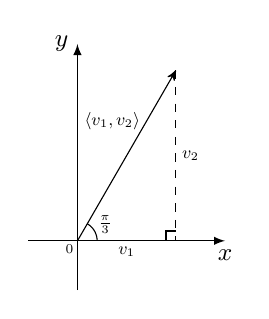
\begin{tikzpicture}[>=latex,xscale=.5*2.5, yscale=.5*2.5][font=\sf\small] 

%\draw[xstep=1cm,ystep=1cm,color=gray!80] (0, -1) grid (8, 8);

    	\foreach \x in {}
     		\draw (\x,2pt/2.5) -- (\x,-2pt/2.5)
			node[anchor=north] {\tiny$\x$}
			;

    	\foreach \x in {}
     		\draw (\x,2pt/1) -- (\x,-2pt/1)
			node[anchor=south] {\tiny$\x$}
			;
    	\foreach \y in {}
     		\draw (-2pt/1,\y) -- (2pt/1,\y)
			node[anchor=east] {\tiny $\y$}
			;

\draw[->] (-0.5, 0) -- (1.5, 0)node[below] {$x$} ;
\draw[->] (0, -0.5) -- (0, 2)node[left] {$y$} ;

\draw[->, >=stealth'] (0, 0) -- (1, {sqrt(3)})node[black, left, midway, pos=0.7, xshift=0, yshift=0, scale=0.7]{$\langle v_1, v_2 \rangle$};

\draw[dashed] (1, {sqrt(3)})--(1, 0)node[black, right, midway, pos=0.5, xshift=0, yshift=0, scale=0.7]{$v_2$};

\node[below, scale=0.7] at (0.5, 0) {$v_1$};

\draw[black, samples=100, smooth, domain=0:pi/3, variable=\t] 
		plot ({0.2*cos(\t r)}, {0.2*sin(\t r)}); 

\draw ({1-0.1}, 0)--++(0, 0.1)--++(0.1, 0); 


\node[xshift = 10, yshift = 5.8, scale=0.7] at (0, 0) {$\frac{\pi}{3}$};

\node[scale=0.7] at (-0.2/2.5, -0.2/2.5) {\scriptsize$0$};

\end{tikzpicture}
\end{document}